\documentclass{beamer}
\usetheme{Singapore}
\usepackage{etex}

\usepackage{listings}
\usepackage{enumerate}
\usepackage[ucs]{}
\usepackage[utf8]{inputenc}
\usepackage[francais]{babel}
\usepackage{graphics}
\usepackage{graphicx}
\usepackage{subcaption}
\usepackage{fancybox}
\usepackage{algorithm,algorithmic}
\usepackage{bbm} 
\usepackage{pstricks}
\usepackage{tikz}
\usepackage{float}
\usepackage[ucs]{}
\usepackage[utf8]{inputenc}
\usepackage[francais]{babel}
\usepackage{amsmath,amssymb,amsfonts,amsthm}
\usepackage{multirow}
\usepackage{color}
\definecolor{grisclair}{rgb}{0.85,0.85,0.85}
\usepackage{graphics}
\usetikzlibrary{arrows,decorations.pathmorphing,backgrounds,fit,positioning,shapes.symbols,chains}

\usetikzlibrary{decorations.pathmorphing}
\usepackage{tkz-euclide}
\usetkzobj{all}

\usepackage{stmaryrd}

%% New commands
\newcommand{\hh}{\ensuremath{\mathbf{\mathcal{H}}} \xspace}
\newcommand{\hmat}{\ensuremath{\mathcal{H}}-matrix \xspace \xspace}
\newcommand{\hmats}{\ensuremath{\mathcal{H}}-matrices\xspace}
\newcommand{\plus}{+}

\newcommand{\vecj}{\ensuremath{\protect \overrightarrow{\mathbf{j}}}\xspace}
\newcommand{\vecm}{\ensuremath{\protect \overrightarrow{\mathbf{m}}}\xspace}
\newcommand{\vecn}{\ensuremath{\protect \overrightarrow{\mathbf{n}}}\xspace}
\newcommand{\veck}{\ensuremath{\protect \overrightarrow{\mathbf{k}}}\xspace}
\newcommand{\vecd}{\ensuremath{\protect \overrightarrow{\mathbf{d}}}\xspace}
\newcommand{\vecom}{\ensuremath{\protect \overrightarrow{\mathbf{w}}}\xspace}

\newcommand{\vecE}{\ensuremath{\mathbf{E}}\xspace}
\newcommand{\vecH}{\ensuremath{\mathbf{H}}\xspace}

\newcommand{\rot}{\ensuremath{\protect \overrightarrow{\mathrm{rot}} }\xspace}
\newcommand{\rotE}{\ensuremath{\protect \overrightarrow{\mathrm{rot}} \, \mathbf{E}}\xspace}
\newcommand{\rotH}{\ensuremath{\protect \overrightarrow{\mathrm{rot}} \, \mathbf{H}}\xspace}

\newcommand{\rotgE}{\ensuremath{\protect \overrightarrow{\mathrm{rot}}_{\Gamma} \, \mathbf{E}}\xspace}
\newcommand{\rotgH}{\ensuremath{\protect \overrightarrow{\mathrm{rot}}_{\Gamma} \, \mathbf{H}}\xspace}
\newcommand{\divgE}{\ensuremath{\mathrm{div}_{\Gamma} \, \mathbf{E}}\xspace}
\newcommand{\divgH}{\ensuremath{\mathrm{div}_{\Gamma} \, \mathbf{H}}\xspace}
\newcommand{\divg}{\ensuremath{\mathrm{div}_{\Gamma} }\xspace}
\newcommand{\divgh}{\ensuremath{\mathrm{div}_{\Gamma_h} }\xspace}
\newcommand{\Div}{\ensuremath{\mathrm{div}}\xspace}
\newcommand{\divE}{\ensuremath{\mathrm{div} \, \mathbf{E}}\xspace}
\newcommand{\divH}{\ensuremath{\mathrm{div} \, \mathbf{H}}\xspace}

\newcommand{\gradg}{\ensuremath{\nabla_{\Gamma} }\xspace}

\newcommand{\vecdpar}{\ensuremath{\protect \overrightarrow{\mathbf{d}_{\parallelslant}}} \xspace}
\newcommand{\vecdperp}{\ensuremath{\protect \overrightarrow{\mathbf{d}_{\bot}}} \xspace}
%\newcommand{\vecdperp}{\ensuremath{\nabla_{\Gamma} }\xspace}

%% d\Gamma(y) for integration
\newcommand{\dg}{\ensuremath{\, \mathrm{d}\Gamma}\xspace}
\newcommand{\mintg}{\ensuremath{\displaystyle \int_{\Gamma}\!}\xspace}
\newcommand{\dgh}{\ensuremath{\, \mathrm{d}\Gamma_h}\xspace}
\newcommand{\mintgh}{\ensuremath{\displaystyle \int_{\Gamma_h}\!}\xspace}
%%


%Affichage graphique
\graphicspath{{./img}}

%En-tete
%\title{Parallel Fast Direct Solver: applications to Uncertainty Management}
%\subtitle{An overview of the \hmat framework}
\title{
Low-rank in Uncertainty Management
}
\subtitle{
Efficient linear algebra and an overview of the $\hmat$ framework
}

\author{Kieran Delamotte}
\institute{IMACS}
\date{May, 2021}

%Insertion des logos
\usepackage{pgf}
\titlegraphic{
%\left
\pgfimage[height=1.2cm]{./img/logoPrace}
%\center
\pgfimage[height=1.2cm]{./img/maisonSimulation}
%\right
\pgfimage[height=1.2cm]{./img/imacs}
}


%Affichage du plan a chaque section et sous-section
\AtBeginSection[]
{
\begin{frame}<beamer>[noframenumbering]

\tableofcontents[currentsection]
\end{frame}
}

\makeatother
\setbeamertemplate{footline}
{
  \leavevmode%
%\hbox{%
  %\begin{beamercolorbox}[wd=.4\paperwidth,ht=2.25ex,dp=1ex,center]{author in head/foot}%
  %  \usebeamerfont{author in head/foot}\insertshortauthor
  %\end{beamercolorbox}%
  \begin{beamercolorbox}[wd=.6\paperwidth,ht=2.25ex,dp=1ex,center]{title in head/foot}%
    \usebeamerfont{title in head/foot}\insertshorttitle\hspace*{1em}
    \insertframenumber{} / \inserttotalframenumber\hspace*{1ex} %%HERE
  \end{beamercolorbox}
}%
  \vskip0pt%
%}
\makeatletter
\setbeamertemplate{navigation symbols}{}

%% header slide
\begin{document}

\begin{frame}%[noframenumbering]
\titlepage
\end{frame}

%%%

\section*{}
\begin{frame}
\tableofcontents
\end{frame}

%% part 0: low rank and random linear algebra
\section{First encounter with low rank}

%%% - intro
\begin{frame}
\frametitle{Key ideas for fast computation}
Uncertainty quantification (UQ) typically requires a high number of simulations using basic linear algebra operations. Then two things come in handy :

  \begin{itemize}
    \item fast linear algebra decomposition ($QR$, $LL^T$, ...)
    \item efficient data strucutures
  \end{itemize}

If many simulations are 'similar' there is most likely a low-rank property somewhere to be exploited. Low-rank property in linear algebra leads to fast computations AND efficient structures!

We shall present two efficient methods :
  \begin{itemize}
    \item random linear algebra for medium-sized problems (on a simple example!)
    \item the $\mathcal{H}$-matrix framework (much more detailed)
  \end{itemize}
\end{frame}


%%% - intro: model problem
\begin{frame}
\frametitle{Model problem}
Suppose we are interested in eigenvalues (and/or eigenvectors) of a covariance matrix of the form $C_X = X^TX$ where X is of size $m \times n$.
Several methods:
  \begin{itemize}
    \item eigenvalue decomposition of $C_X$: $\mathcal{O}(n^3)$ operations and conditionning of normal equations is bad!
    \item SVD decomposition of X: (better, still expensive) $\mathcal{O}(mn^2)$ operations
    \item \alert{what else?}
  \end{itemize}
\end{frame}

%%% - random QR
\begin{frame}
\frametitle{Randomness and linear algebra}
\textbf{Basic idea:} using random test matrix $\Omega$ and the fact that any orthogonal basis of $\mathrm{ran}(Y)$ with $Y=A \Omega$ is a good approximate basis for $\mathrm{ran}(A)$. $Y$ has a less columns than $A$ so $QR$ is cheaper! 

  \begin{algorithm}[H]
  \caption{A simple random QR decomposition}
  \label{rQR}
  \begin{algorithmic}[1]

  \REQUIRE A matrix $\mathbf{A}$ of size $m \times n$, an oversampling parameter $l$.
  \ENSURE An orthogonal basis $\mathbf{Q_Y}$ of $\mathrm{ran}(\mathbf{A})$. 

  \STATE Draw a random matrix $\mathbf{W}$ of size $n \times l$.
  \STATE Form product $\mathbf{Y}$ : $\mathbf{Y} = \mathbf{A} \mathbf{W}$. 
  \STATE Form the $QR$ decomposition of the matrix $\mathbf{Y}$ : $\mathbf{Y}=\mathbf{Q_Y} \mathbf{R}$.
  \RETURN
  \end{algorithmic}
  \end{algorithm}
\end{frame}


%%% - random SVD
\begin{frame}
\frametitle{A random SVD}
  \begin{algorithm}[H]
  \caption{A simple random SVD decomposition}
  \label{rSVD}
  \begin{algorithmic}[2]
  \REQUIRE A matrix $\mathbf{A}$ of size $m \times n$, an orthogonal matrix $\mathbf{Q}$ tq $\mathbf{A} \simeq \mathbf{Q}\mathbf{R}$.
  \ENSURE An approximate $SVD$ decomposition of $\mathbf{A}$, $\mathbf{A} \simeq \mathbf{U} \mathbf{\Sigma} \mathbf{V}^T$.

  \STATE Construct the projection matrix $\mathbf{B}=\mathbf{Q}^T \mathbf{A}$.
  \STATE Form the SVD of $\mathbf{B}$ : $\mathbf{B} = \mathbf{\tilde{U}} \mathbf{\Sigma} \mathbf{V}^T$. 
  \STATE Build the matrix $\mathbf{U} = \mathbf{Q} \mathbf{\tilde{U}}$.

  \RETURN
  \end{algorithmic}
  \end{algorithm}
\end{frame}


%%% - a numerical example
\begin{frame}
\frametitle{A numerical example}

Say $X \in \mathbb{R}^{m \times n}$ is a discrete approximate of a random process $X(t,\omega)$ over $[-1,1]$ with exponential covariance function $C(s,t) = e^{-|t-s|}$. We are still interested in eigenvalues of $C_X$. In that case, we can prove that $\lambda_n / \lambda_1 = \mathcal{O}(n^{-2})$.

In the following example we choose $m=6400$ and $n=1000$.
\end{frame}

%%% - Eigenvalues profile
\begin{frame}
\frametitle{Eigenvalues estimates}

\begin{columns}[t]
  \begin{column}{5cm}
\begin{figure}[H]
\begin{center}
  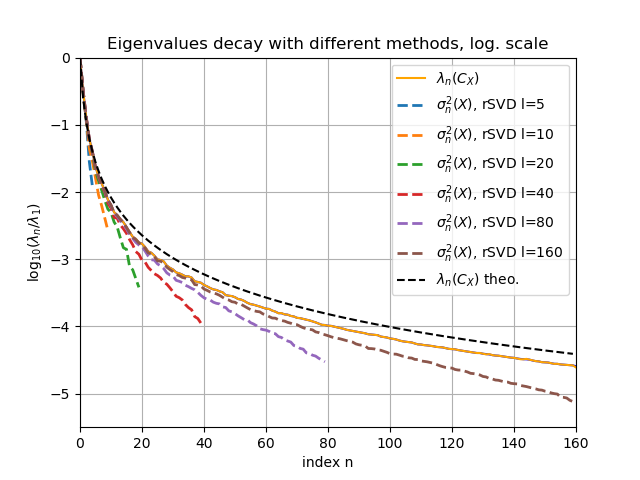
\includegraphics[scale=0.3]{./img/eigenValues_1.png}
  \caption{Eigenvalues decay.}
\end{center}
\end{figure}

\end{column}
  
  \begin{column}{5cm}
    \begin{figure}[H]
    \begin{center}
  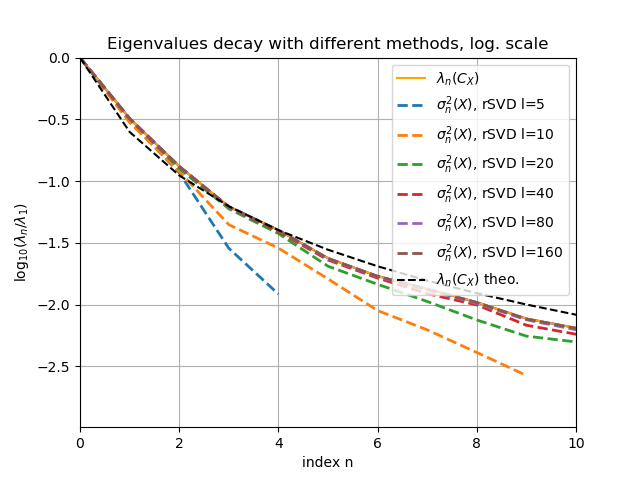
\includegraphics[scale=0.3]{./img/zoom-1.png}
  \caption{Eigenvalues decay - the first 10.}
     \end{center}
     \end{figure}

  \end{column}
 \end{columns}  
\end{frame}

%%% - Timings
\begin{frame}
\frametitle{Case summary}
\begin{table}[H]
\centering
\begin{tabular}{rrrr}
\hline
test matrix \# cols.  & elapsed time (s) &   $\sum \lambda_n$ & rel. error \\
\hline
               5 & 0.021            & 4950345.8          & 0.253      \\ 
              10 & 0.027            & 5894250.4          & 0.111      \\ 
              20 & 0.038            & 6309314.4          & 0.048      \\
              40 & 0.060            & 6478969.3          & 0.023      \\
              80 & 0.068            & 6556588.8          & 0.011      \\ 
             160 & 0.131            & 6598333.6          & 0.005      \\
\hline
\end{tabular}
\caption{Example summary for random SVD \label{tab:rSVD}}                
\end{table}

\begin{itemize}
  \item For reference : $\mathrm{trace}(C_X) = 6632269.0$
  \item elapsed time for full SVD: 0.663s
  \item elapsed time for \textit{numpy.linalg.eigs}: 107.307.
\end{itemize}
\end{frame}

%%% - Partial conclusion
\begin{frame}
\frametitle{Partial conclusion}
\begin{itemize}
  \item many articles in the literature,
  \item random SVD is implemented in OPENTURNS,
  \item generally behave better than classical methods,
  \item \alert{what if the problem is larger ?}
\end{itemize}
\end{frame}


%% part 1: simple Kriging intro
\section{Large and dense systems}
\begin{frame}
\frametitle{Introduction}
Several applications in statistics lead to large and dense matrices:
\begin{itemize}
\item Karhunen-Loève decomposition;
\item Kriging;
\item applications using large covariance matrices (ex: random Gaussian sampling).
\end{itemize}

\begin{block}{Covariance matrices}
Let $Z:\mathbb{R}^d \mapsto \mathbb{R}$ be some random process, stationnary of 
order 2. We have N observation points $\left\{ x_i \in \mathbb{R}^d /i=1,\hdots,N \right\}$ with values $Z(x_i)$.
Let assume that the covariance of these points is known and given by a matrix $K \in \mathbb{R}^{N \times N}$ with

\[ K_{ij} = \mathrm{Cov}(Z(x_i),Z(x_j)) \]
%\begin{itemize}
%\item Symetric Positive Definite (SPD) matrix;
%\item Many solves;
%\item Usually,
% \begin{itemize}
%  \item Cholesky decomposition $K=LL^T$;
%  \item Forward/Backward substitutions.
% \end{itemize}
%\end{itemize}
\end{block}
\end{frame}

%\begin{frame}
%\frametitle{Covariance matrices}
%\framesubtitle{}
%
%Let $Z:\mathbb{R}^d \mapsto \mathbb{R}$ be some random process, stationnary of 
%order 2. We have N observation points $\left\{ x_i \in \mathbb{R}^d /i=1,\hdots,N \right\}$ with values $Z(x_i)$.
%Let assume that the covariance of these points is known and given by a matrix $K \in \mathbb{R}^{N \times N}$ with
%
%\[ K_{ij} = \mathrm{Cov}(Z(x_i),Z(x_j)) \]
%
%\end{frame}

\begin{frame}
\frametitle{Covariance matrices}
\framesubtitle{covariance kernel}

%Consider a covariance matrix $K$.
\begin{itemize}
  %\item $K$ is SPD (covariance matrix);
  \item usually $K$ is not known exactly:
    \begin{itemize}
    \item modelled as a convolution matrix of a kernel $k: \mathbb{R}^d \mapsto \mathbb{R}_{\plus}$:
       \[ K_{ij} := k(x_i,x_j) \]
    \item what is $k$?
    \begin{itemize}
      \item Exponential:
       \[ k(x,y) = e^{-|x-y|/\lambda} \]
      \item Gaussian:
       \[ k(x,y) = e^{-|x-y|^2/(2\lambda^2)} \]
      \item Quadratic:
       \[ k(x,y) = \left(1+\frac{|x-y|}{2 \lambda} \right)^{-2}  \]
      \item and many more!
    \end{itemize}
 \end{itemize}

  \item N can be large. For instance, every node in a FEM discretization;
\end{itemize}
\end{frame}

\begin{frame}
\frametitle{Covariance matrices}
\framesubtitle{linear algebra}
\begin{itemize}
\item K is ill-conditionned, many RHS: direct solver;
\item K is SPD: Cholesky.
\end{itemize}

\begin{block}{Complexity (LAPACK)}
  \begin{itemize}
    \item Cholesky factorization (DPOTRF): $1/3N^3 + 1/2N^2 + 1/6N$
    \item Solving (DPOTRS): $N_{\mathrm{RHS}} \times 2N^2$
    \item Storage: $8N^2/2$
  \end{itemize}
\end{block}
\alert{Need of a fast direct solver: \hmat framework.}
\end{frame}

\begin{frame}
\frametitle{Toy model: exponential kernel in 1D}
Let $X_N$ be a uniform discretization of $[0,1]$ with the 
discretization step $h = \frac{1}{N-1}$ : 

\[ X_N = \left\{ 0=x_1,\hdots,x_N=1\right\} 
\]

The correlation length $\lambda$ is set to $\lambda:=5h$ and the exponential kernel in 1D reads as 

\[ K_{\lambda}(x_i,x_j) = e^{-|x_i-x_j|/\lambda} 
\]
\end{frame}


\begin{frame}
\frametitle{Toy model: exponential kernel in 1D}
\only<1|handout:4>{
\begin{figure}
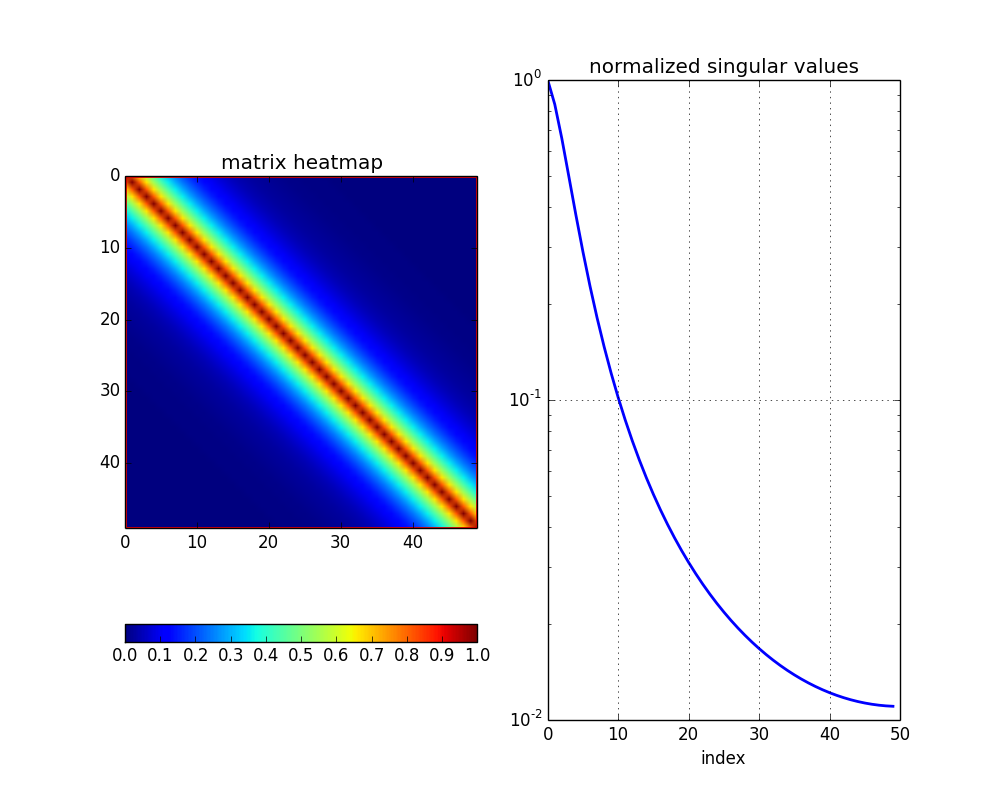
\includegraphics[scale=0.3]{./img/original_matrix_exp_1d.png}
\caption{the covariance matrix $K_{\lambda}([0,1],[0,1])$}
\end{figure}
}
\only<2|handout:4>{
\begin{figure}
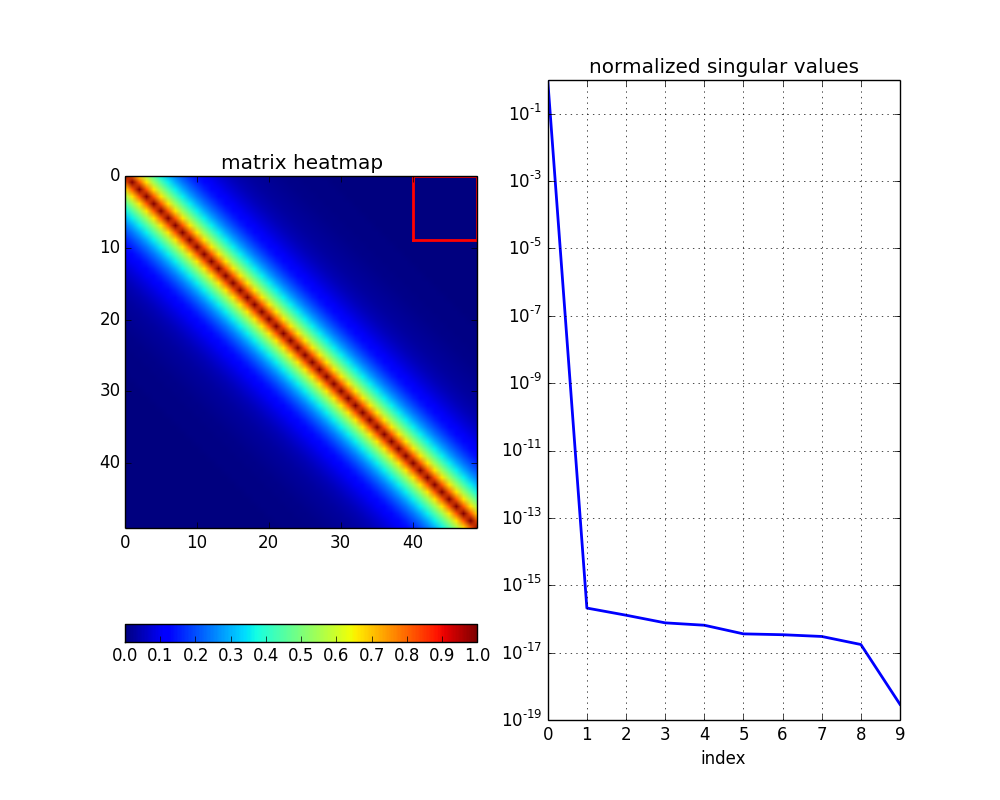
\includegraphics[scale=0.3]{./img/original_matrix_exp_1d_small.png}
\caption{small extra-diagonal block: $K_{\lambda}([0,0.2],[0.8,1])$ }
\end{figure}
}
\only<3|handout:4>{
\begin{figure}
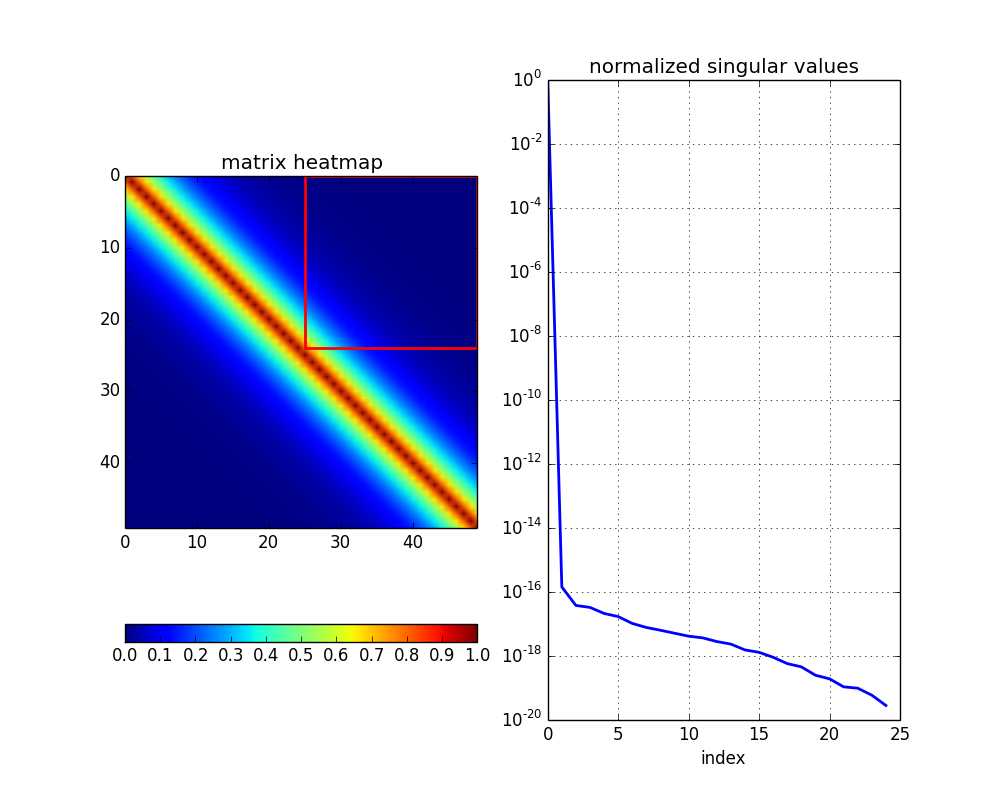
\includegraphics[scale=0.3]{./img/original_matrix_exp_1d_big.png}
\caption{large extra-diagonal block: $K_{\lambda}([0,0.5],[0.5,1])$ }
\end{figure}
}
\only<4|handout:4>{
\begin{figure}
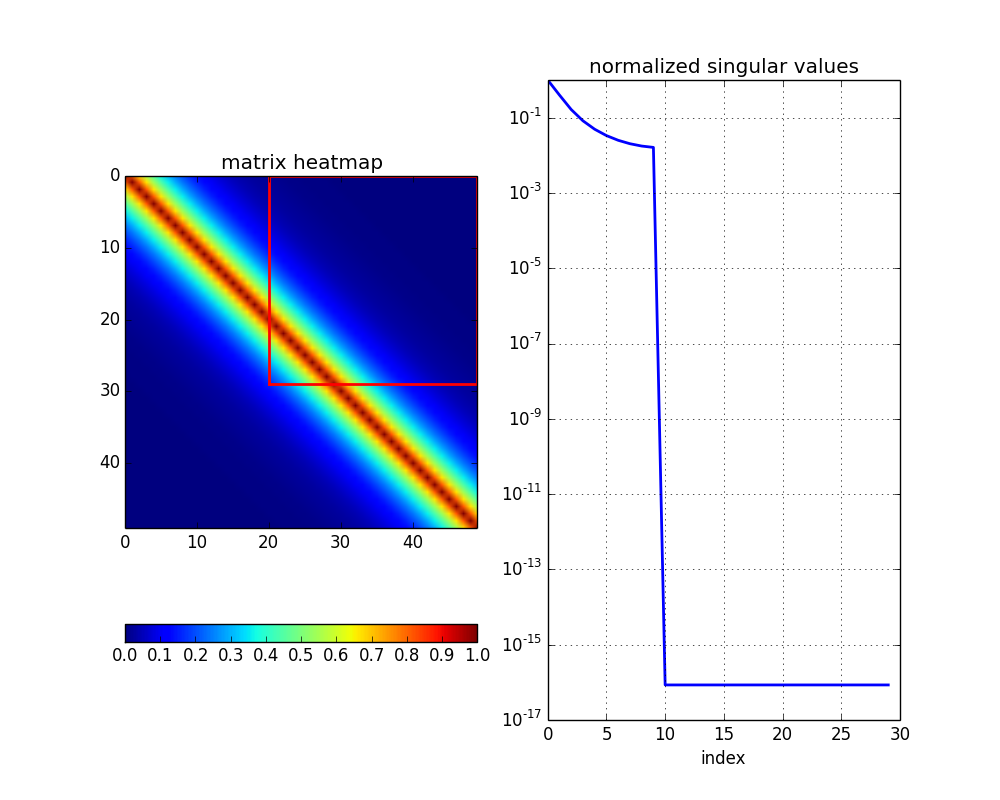
\includegraphics[scale=0.3]{./img/original_matrix_exp_1d_diag.png}
\caption{taking a part of the diagonal: $K_{\lambda}([0,0.6],[0.4,1])$ }
\end{figure}
}
\end{frame}

\begin{frame}
\frametitle{Toy model: exponential kernel in 1D}
Whenever $x_i$ and $x_j$ are in disjoint sets the kernel reads as a separated one. For instance; if $x_i > x_j$ then 

\[ K_{\lambda}(x_i,x_j) = e^{(x_j-x_i)/\lambda} = e^{x_j/\sqrt{\lambda}}e^{-x_i/\sqrt{\lambda}} , 
\]
which is of rank 1.
\end{frame}



%% part 2: the H-matrix framework
\section{$\hmats$}

\begin{frame}
\frametitle{Admissibility gives low-rank}

\begin{figure}%[scale=0.8]
\begin{tikzpicture}[scale=0.7]
\draw[thick] (4,1) rectangle (5,2);
\draw[thick] (7,3) rectangle (8,5);
\draw[thick,<->,dashed,red] (4,1) -- (5,2);
\draw[thick,<->,dashed,red] (7,3) -- (8,5);
\draw[thick,red] (5.2,1.5) node[right]{$\mathrm{diam}(B_s)$};
\draw[thin,red,<-] (4.5,1.5)--(5.2,1.5);
\draw[thick,red] (6.8,4) node[left]{$\mathrm{diam}(B_t)$};
\draw[thin,red,->] (6.8,4)--(7.5,4);
\draw[thick,<->] (5,2) -- (7,3);
\draw[thick] (7.4,2.5) node[below]{$\mathrm{dist}(B_s,B_t)=R$};
\draw[thick] (4.5,1) node[below]{$B_s$};
\draw[thick] (7.5,5) node[above]{$B_t$};

\fill[blue] (4.1,1.7) circle[radius=2pt];
\fill[blue] (4.65,1.18) circle[radius=2pt];
\fill[blue] (4.8,1.54) circle[radius=2pt];
\fill[blue] (4.9,1.67) circle[radius=2pt];
\fill[blue] (4.34,1.24) circle[radius=2pt];

\fill[blue] (7.2, 3.67) circle[radius=2pt];
\fill[blue] (7.5, 4.18) circle[radius=2pt];
\fill[blue] (7.80, 3.90) circle[radius=2pt];
\fill[blue] (7.13, 4.50) circle[radius=2pt];
\fill[blue] (7.67, 3.27) circle[radius=2pt];


  \draw[thick=1] (9,4) rectangle (11,6);
  \fill[red!60!white] (9,4) rectangle (11,6);
  \node at (10.0,5.0) {$M$};
  \node[above] at (11.3,5.0) {$\approx$};
  \node[left] at (9.0,5.0) {$m$};
  \node[above] at (10.0,6.0) {$n$};



  \draw[thick] (11.6,4) rectangle (12.0,6.0);
  \fill[green!60!white](11.6,4) rectangle (12.0,6.0);
  \node at (11.8,5.0) {$A$};
  \node[left] at (11.6,4.6) {$m$};
  \node[above] at (11.8,6.0) {$r$};



  \draw[thick] (12.6,5.6) rectangle (14.6,6.0);
  \fill[green!60!white](12.6,5.6) rectangle (14.6,6.0);
  \node at (13.6,5.8) {$B^T$};
  \node[right] at (14.6,5.8) {$r$};
  \node[above] at (13.6,6.0) {$n$};

\end{tikzpicture}
\end{figure}

Usual condition:
\[
\min(\mathrm{diam}(B_t),\mathrm{diam}(B_s)) \leqslant \eta \, \mathrm{dist}(B_t,B_s) \qquad \text{(admissibility condition)}
\]

The separation condition $R=0$ gives the \textbf{HODLR}(\textbf{H}ierarchically \textbf{O}ff-\textbf{D}iagonal \textbf{L}ow-\textbf{R}ank) structure described by the 1D toy model.
\end{frame}


\begin{frame}
\frametitle{Low-rank approximation: compression techniques}
\begin{itemize}
\item SVD: $M \approx U \Sigma V^H$
\begin{itemize}
\item Rank and precision controlled;
\item {\color{red}Costly $\mathcal{O}(4m^2n+8mn^2+9n^3)$} (hyp: $m>n$)
\end{itemize}
\item Existence of cross approximations: row/col. extraction (Goreinov \& Tyrtyshnikov '97);
\item Gaussian/LU rank-revealing scheme known as \textbf{Full Cross Approximations}:
\floatname{algorithm}{Algorithme}
\begin{algorithm}[H]
\begin{algorithmic}[1]
\WHILE{$ \lVert M \rVert \geq {\varepsilon} \lVert M_0 \rVert $:}
    \STATE $\mathrm{rank}(M) \leftarrow \mathrm{rank}(M) + 1$
    \STATE Find the coefficient $M_{i^{\star}j^{\star}}$ so that $M_{i^{\star}j^{\star}}=\max_{i,j}|M_{ij}|$, $\alpha = M_{i^{\star}j^{\star}}$
    \STATE $M \leftarrow M-\frac{1}{\alpha}M(:,j^{\star})M(i^{\star},:)$
\ENDWHILE
\end{algorithmic}
\end{algorithm}
\end{itemize}
\end{frame}

\begin{frame}
\frametitle{Variants} 
The fast determination of the pivot is
the main idea of all fast algorithms. Key points to speed up the full cross approximation:
\begin{itemize}
\item \textbf{Partially pivoted Cross Approximation}.
\begin{itemize}
\item We seek the largest pivot over a column and/or a row in $\mathcal{O}(m)$ instead of $\mathcal{O}(m^2)$ operations. 
\item Only the modified coefficients of the remainder are computed at each step.
\end{itemize}

\item \textbf{Adaptive CA algorithm} : a fast (linear) estimation of the remainder.
\item \textbf{ACA+} and other variants use other heuristics.
\item Trade-off between robustness (SVD) and efficiency (ACA/ACA+): computations from {\color{red}$\mathcal{O}(m^2n+mn^2)$}(SVD) to {\color{red}$\mathcal{O}(mnr)$}(fullCA) to {\color{red}$\mathcal{O}((m+n)r^2)$}(ACA).
\end{itemize}
\end{frame}


\begin{frame}
\frametitle{Space partitioning: clustering}
\only<1|handout:5>{
\begin{itemize}
\item Use of \textbf{bounding boxes}: easier to handle than point clouds;
\item Recursive splitting strategy (\textbf{Divide and Conquer strategy}) thanks to \textbf{nested bisection}: 
\begin{itemize}
\item geometric: the box is split in two halves along the largest axis;
\item median: each half contains roughly the same number of unknowns;
\item others (PCA,...).
\end{itemize}
\item Split the boxes until each box contains a fixed small number of unknowns;
\item Result: \textbf{binary tree}.
\end{itemize}
}
\only<2|handout:5>{
\begin{figure}[H]
    \begin{center}
  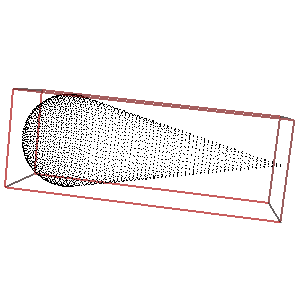
\includegraphics[scale=0.4]{./img/geometric_01}
  \caption{Illustration of the geometric clustering on a cone-sphere.}
     \end{center}
     \end{figure}
}
\only<3|handout:5>{
\begin{figure}[H]
    \begin{center}
  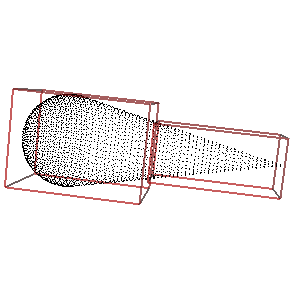
\includegraphics[scale=0.4]{./img/geometric_02}
  \caption{Illustration of the geometric clustering on a cone-sphere.}
     \end{center}
     \end{figure}
}
\only<4|handout:5>{
\begin{figure}[H]
    \begin{center}
  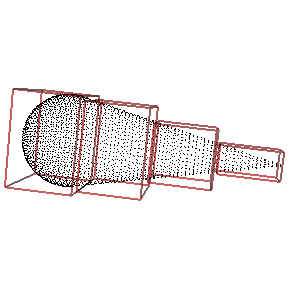
\includegraphics[scale=0.4]{./img/geometric_03}
  \caption{Illustration of the geometric clustering on a cone-sphere.}
     \end{center}
     \end{figure}
}
\only<5|handout:5>{
\begin{figure}[H]
    \begin{center}
  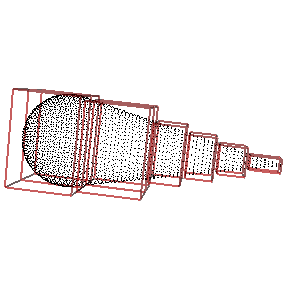
\includegraphics[scale=0.4]{./img/geometric_04}
  \caption{Illustration of the geometric clustering on a cone-sphere.}
     \end{center}
     \end{figure}
}
\end{frame}

\begin{frame}
\frametitle{Blockclustering: Clustering \& Admissibility}
It is a quad-tree whose nodes are matrix blocks and the leaves are admissible (or small) blocks; a block is split in a $2 \times 2$ block structure. 
\begin{table}[ht]
\centering
\begin{tabular}{cc}
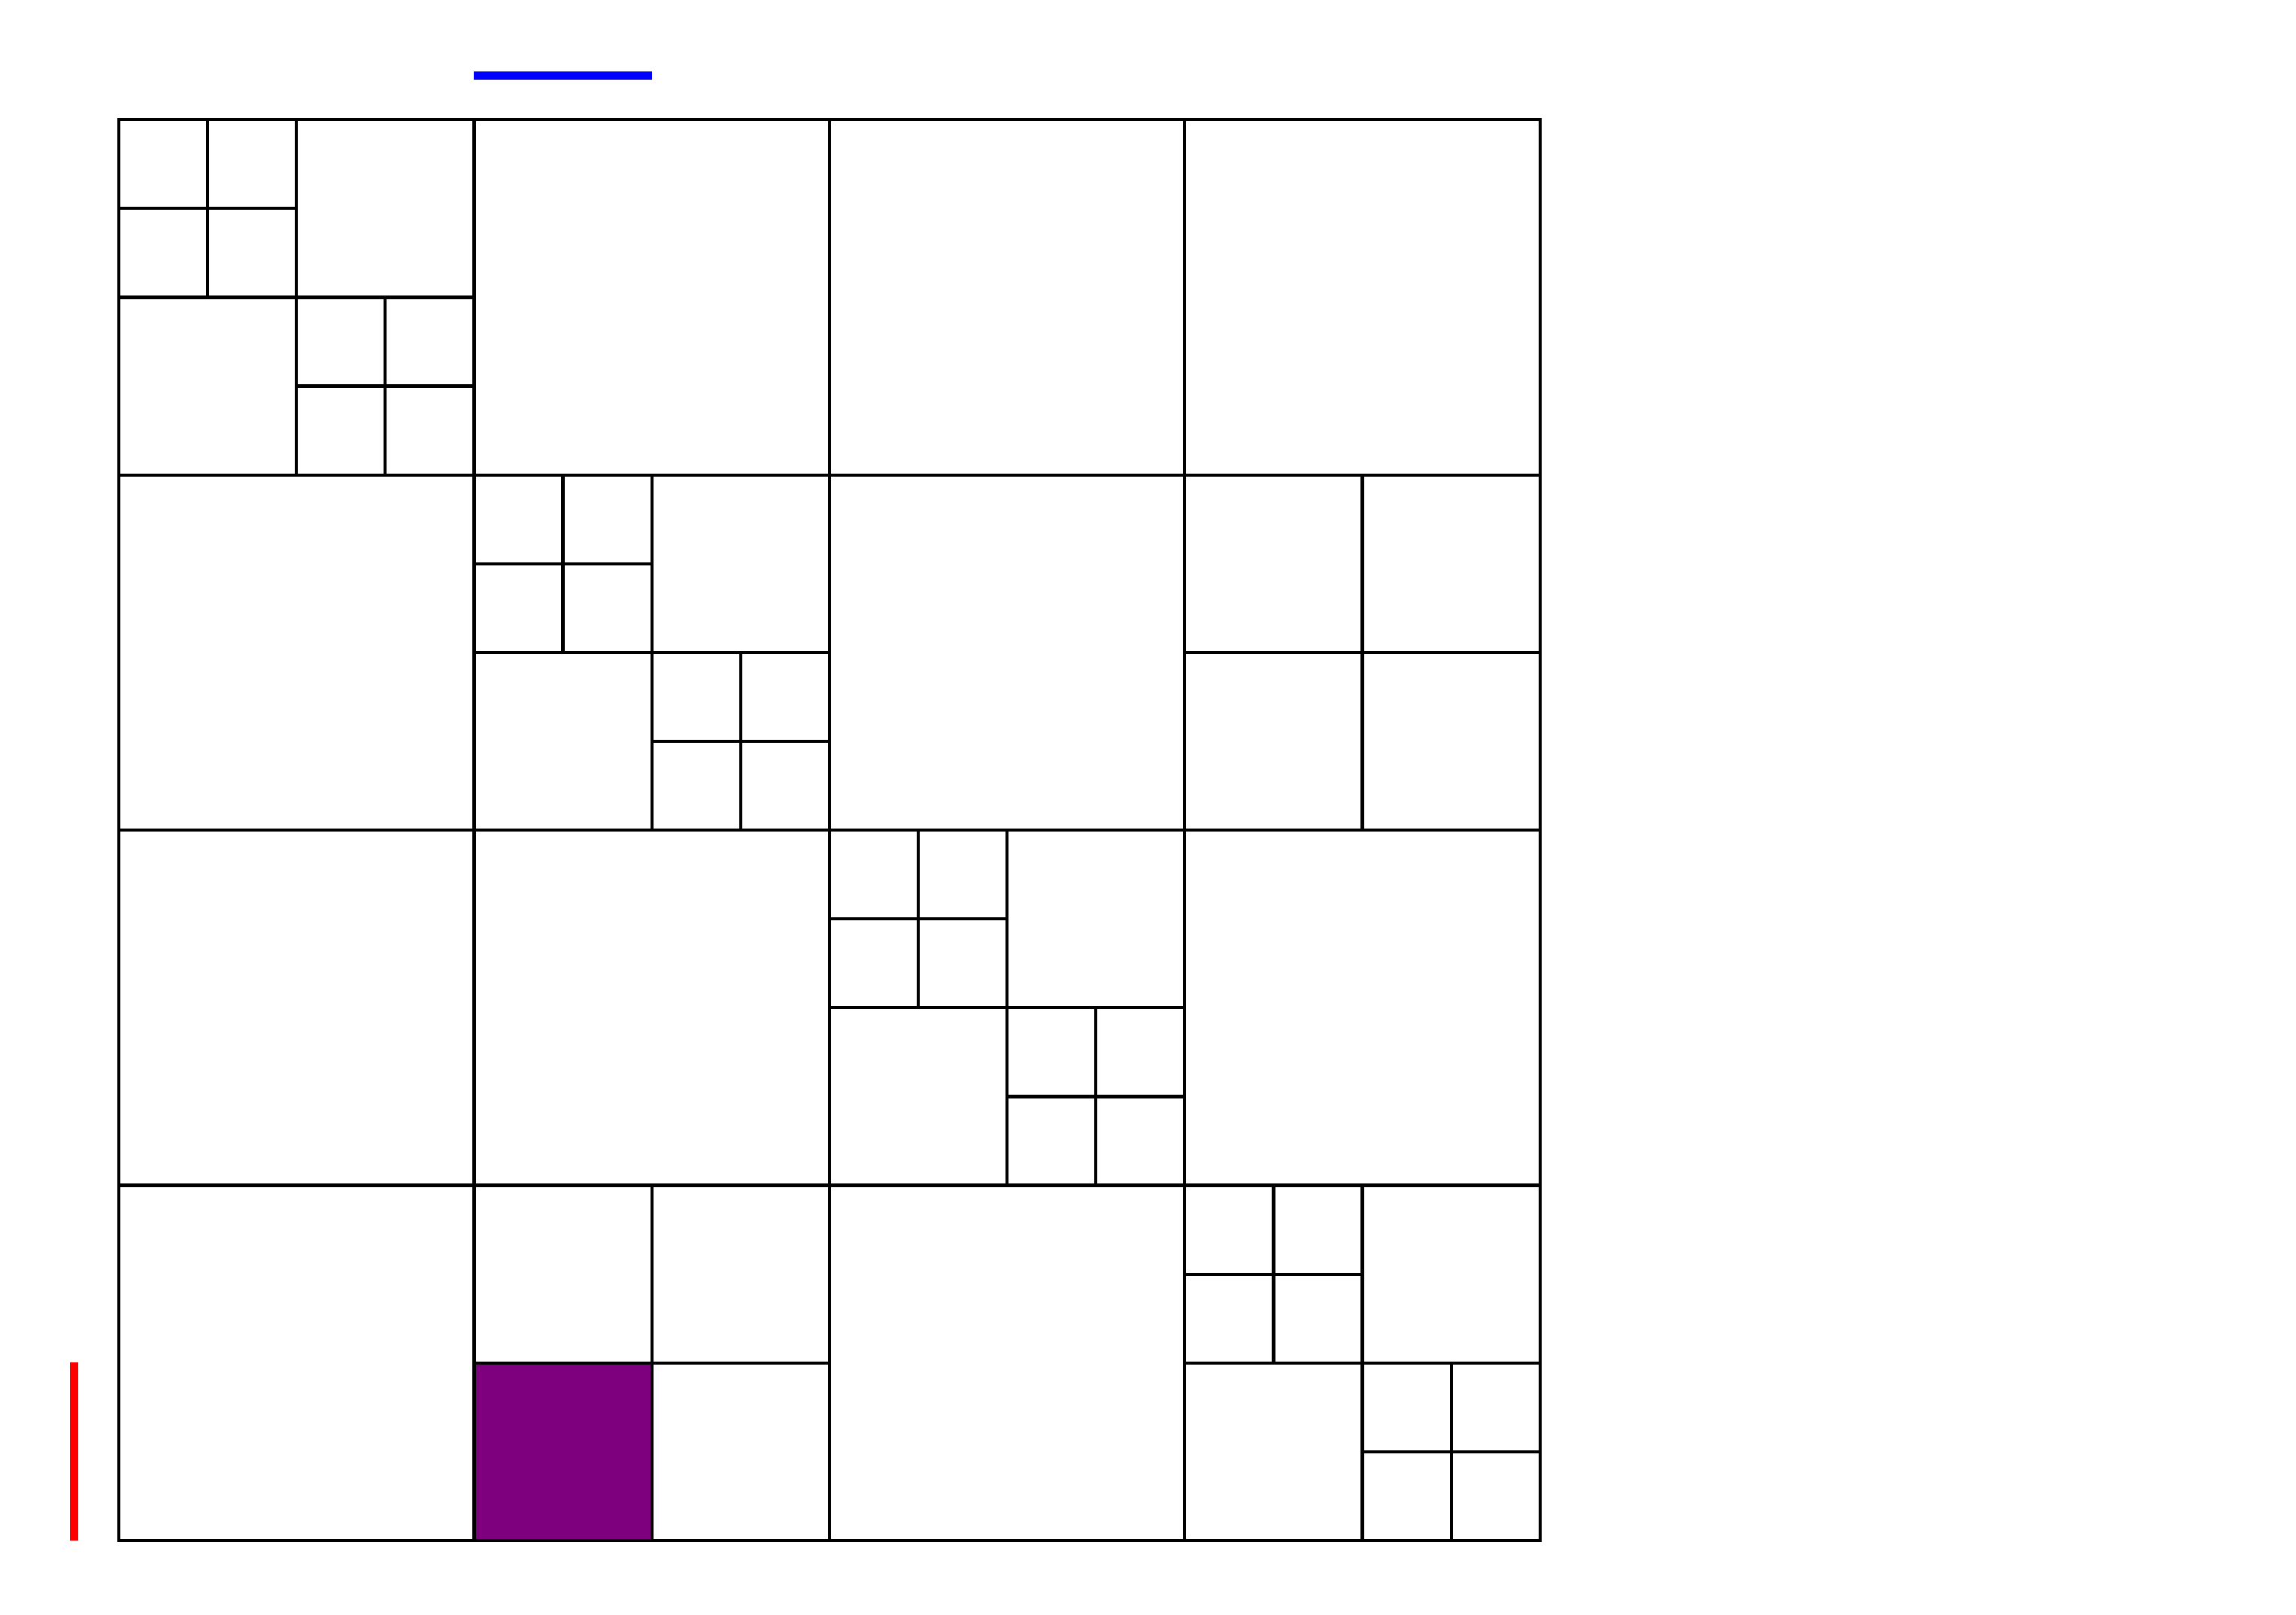
\includegraphics[scale=0.4]{./img/BlockClusteringA.png} & 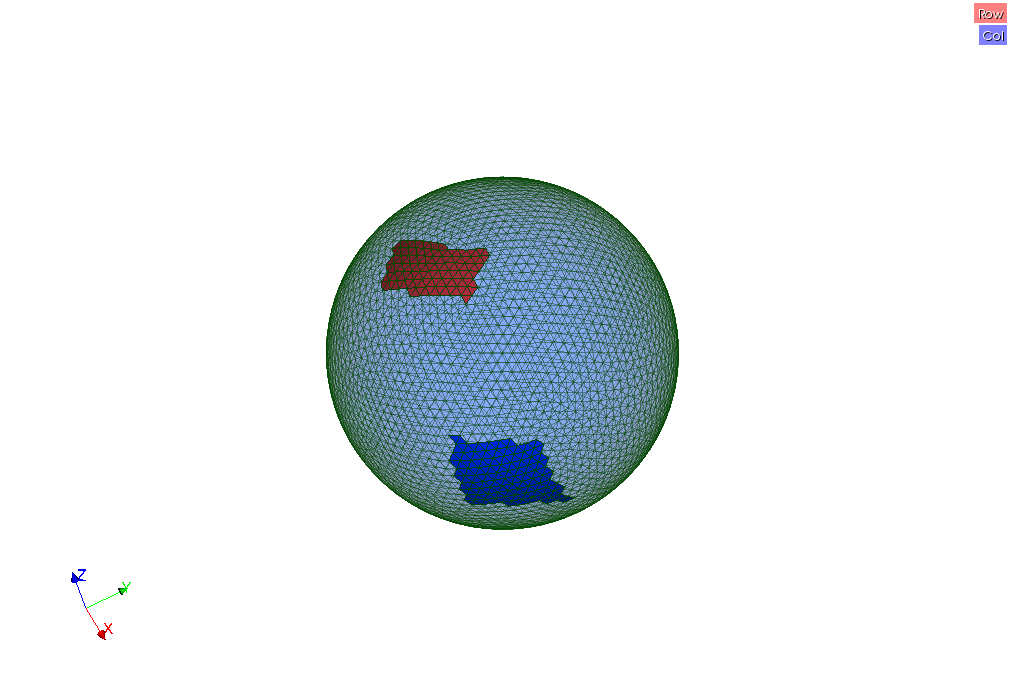
\includegraphics[scale=0.244]{./img/BlockClusteringB.png}
\end{tabular}
\caption{Blockclustering and the geometry}
\end{table}
\end{frame}

\begin{frame}
\frametitle{The \hmat structure}

A \hmat  is a \textbf{quadtree} (with Binary Space Partitioning):
\begin{itemize}
\item Internal nodes: subdivided \hmat; 
\item Leaves:
\begin{itemize}
\item admissible block: large \& low-rank;
\item inadmissible block: dense \& full rank, but small.
\end{itemize}

\begin{block}{Remarks}
\begin{itemize}
\item Only the leaves carry data; 
\item Big admissible blocks ($10^4 \times 10^4$ and more)
\item Small (and few) inadmissible blocks ($100 \times 100$).
\end{itemize}
\end{block}

\end{itemize}

Each admissible block is compressed with a fast method thus determining a numerical rank with  a prescribed relative error {$\varepsilon$}.

\end{frame}


\begin{frame}
\frametitle{Operations: three kinds}

\begin{itemize}
  \item \textbf{\hh-BLAS1\&2:} Assembly, AXPY, GEMV \newline
        Simple. Operating only on leaves.
  \item \textbf{\hh-BLAS3:} GEMM, TRSV \newline 
        More involved. Operations at many different levels of the same sub-tree.
  \item \textbf{\hh-LAPACK:} Inverse, $LU$, $LL^T$.\newline
        Uses BLAS2 and BLAS3 operations, harder to implement in parallel.
\end{itemize}

\begin{block}{Base operations}
All operations use BLAS/LAPACK. Typical subroutines are: SVD, QR, 
LU, TRSV, GEMM and GEMV.
\end{block}
\end{frame}

%%%

\begin{frame}
\frametitle{Computation details}
\begin{block}{Typical issues}
The \hmat algorithms are not nice for the hardware:
\begin{itemize}
\item Very small operations; 
\item Oddly-shaped matrices: "Tall \& skinny";
\item High memory band.
\end{itemize}
\end{block}

\begin{block}{Observations}
  \begin{itemize}
    \item Most (70-80\%) of the time spent in: 
    \begin{itemize}
      \item QR decompositions of T\&S matrices; 
      \item SVD decompositions of small matrices.
    \end{itemize}
    \item BLAS implementions cannot reach the peak performance;
    \item Very high memory bandwidth.
  \end{itemize}
\end{block}
\end{frame}

%%%

\begin{frame}
\frametitle{Complexity estimates}

\begin{alert}{Useful pointers}
\begin{itemize}
\item Most complexity estimates assume a fixed upper bound $k$ for the 
low-rank matrices involved;
\item The structure of the matrix (as represented by a tree) is 
important as well: a large depth with small blocks is typically a bad omen.
\end{itemize}
\end{alert}

\begin{block}{Common operations}
For a matrix size of $N \times N$ with the previous assumptions:
\begin{itemize}
\item assembly:  time and storage is in $\mathcal{O}(kN \log N)$;
\item addition: $\mathcal{O}(k^2N \log N )$ operations;
\item multiplication and Cholesky factorisation: $\mathcal{O}(k^3 N \log^3 N )$ operations;
\item \textcolor{red}{in practice a $\mathcal{O}(N \log^2 N)$ complexity is observed.}
\end{itemize}
\end{block}

\end{frame}



%% part 2: some results
\section{Applications}

%% 1D
\begin{frame}
\frametitle{Recall the 1D toy model?}

\only<1|handout:4>{
\begin{itemize}
  \item exponential kernel: $K(s,t) = e^{-|s-t|/\lambda}$
  \item prescribed relative error $\varepsilon=10^{-4}$;
  \item \textbf{HODLR} admissibility;
  \item 1D exponential kernel: provably rank-one when \textbf{HODLR}.
  \item 'exact model' is the second Hermite function $\psi_2(x) = (2x^2-1)e^{-\frac{1}{2}x}$;
  \item input data as a gaussian distribution;
  \item here: one iteration of optimization loop, correlation length $\lambda=0.01$.
\end{itemize}
}

\only<2|handout:4>{
\begin{figure}[H]
\begin{center}
  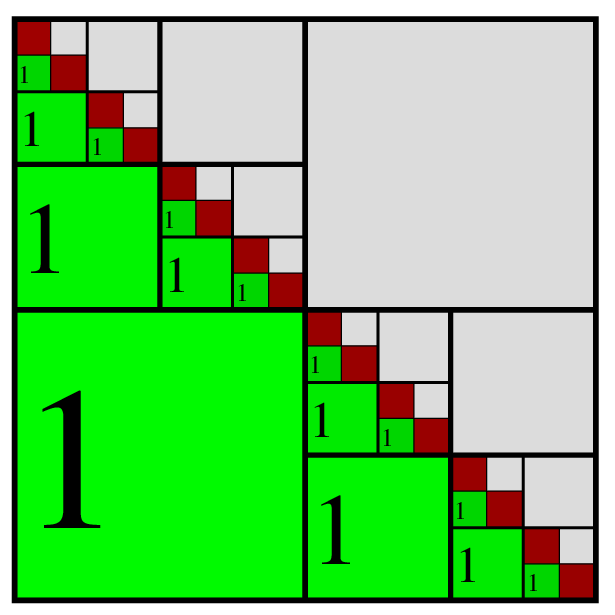
\includegraphics[scale=0.23]{./img/hmatrix-exp1d-assembled}
  \caption{Lower part of the covariance matrix: rank map.}
\end{center}
\end{figure}
\begin{itemize}
\item matrix size $1000 \times 1000$;
\item compression ratio: $\approx 12\%$ \textcolor{red}{(small case!)}
\end{itemize}
}

\only<3|handout:4>{
\begin{figure}[H]
\begin{center}
  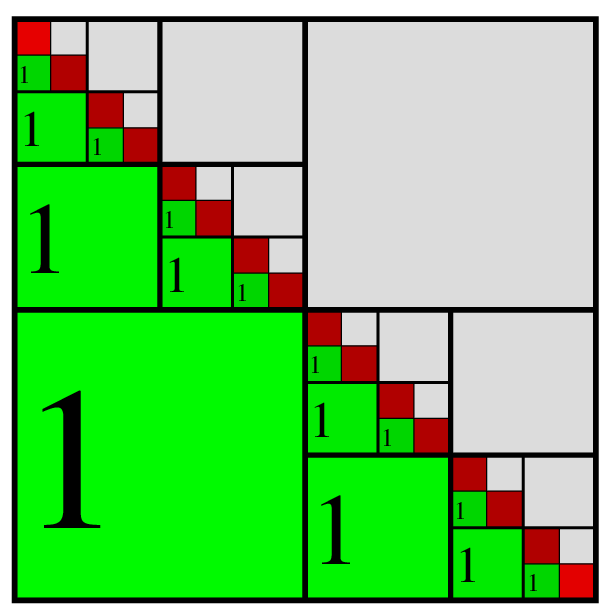
\includegraphics[scale=0.23]{./img/hmatrix-exp1d-factorized}
  \caption{Cholesky factor: rank map.}
\end{center}
\end{figure}
\begin{itemize}
\item matrix size $1000 \times 1000$;
\item compression ratio: $\approx 12\%$ \textcolor{red}{(small case!)}
\end{itemize}
}

\only<4|handout:4>{
\begin{figure}[H]
\begin{center}
  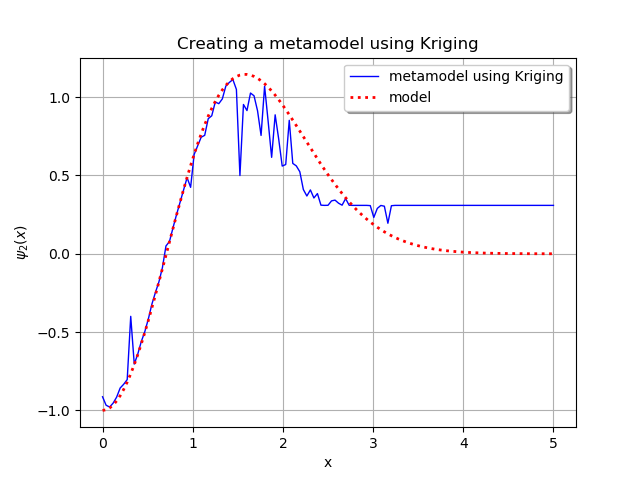
\includegraphics[scale=0.35]{./img/krigingResponse1d}
  \caption{Surface response using kriging}
\end{center}
\end{figure}

\begin{itemize}
\item compression ratio: $\approx 12\%$ \textcolor{red}{(small case!)};
\item same response with LAPACK and HMAT solver;
\item maximum absolute error between two approximates: $1.55 \times 10^{-15}$.
\end{itemize}
}
\end{frame}


%%%% time
\begin{frame}
\frametitle{Performances - computational time}
\framesubtitle{the exponential kernel in 1D}
\begin{figure}
    \centering
    \begin{subfigure}[b]{0.45\textwidth}
        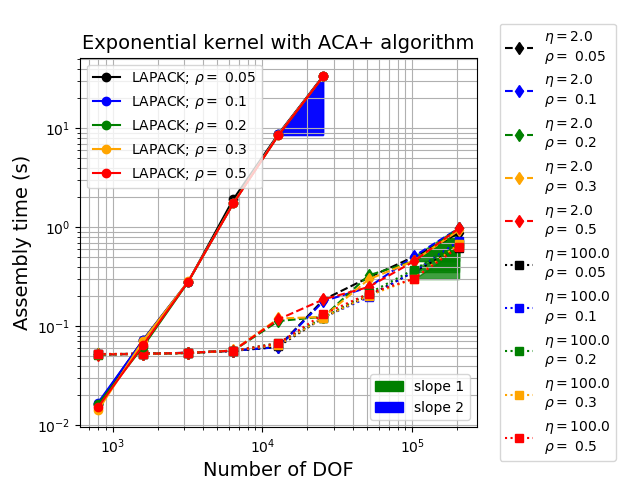
\includegraphics[scale=0.3]{./img/line_EXP_assembly_time}
        \caption{Matrix assembly}
    \end{subfigure}
    \begin{subfigure}[b]{0.45\textwidth}
        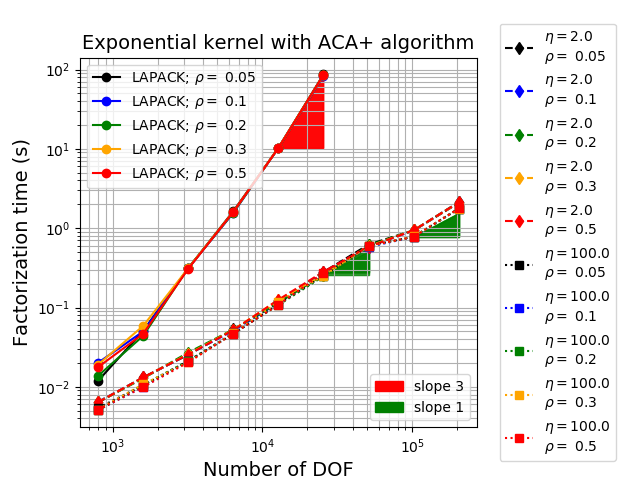
\includegraphics[scale=0.3]{./img/line_EXP_factorization_time}
        \caption{Matrix factorization}
    \end{subfigure}
    \caption{Computational time vs matrix size}
\end{figure}
\end{frame}

%%%% memory
\begin{frame}
\frametitle{Performances - memory}
\framesubtitle{the exponential kernel in 1D}
\begin{figure}
    \centering
    \begin{subfigure}[b]{0.45\textwidth}
        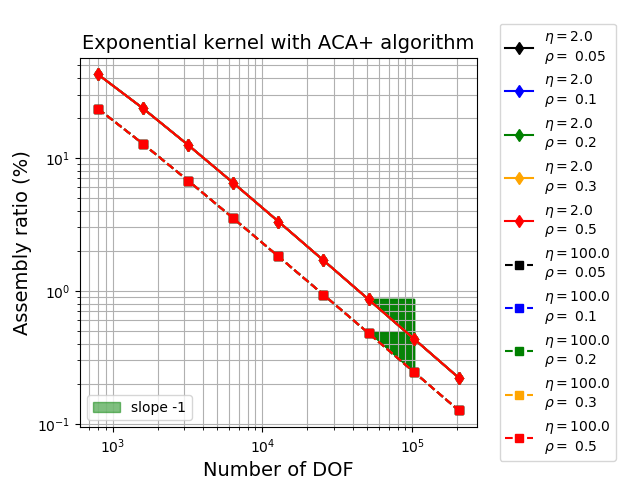
\includegraphics[scale=0.3]{./img/line_EXP_assembly_ratio}
        \caption{Matrix assembly}
    \end{subfigure}
    \begin{subfigure}[b]{0.45\textwidth}
        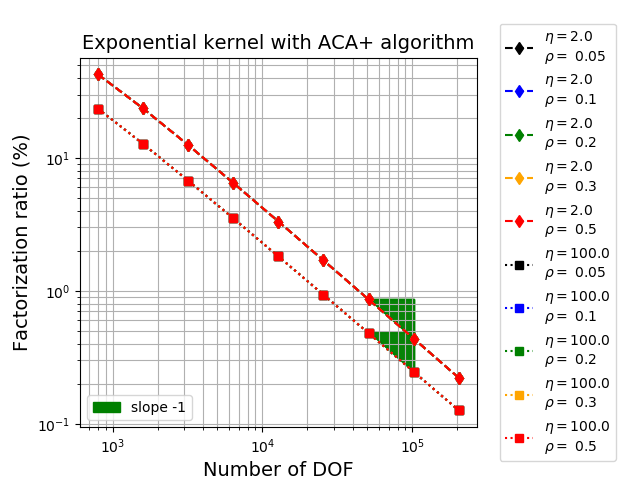
\includegraphics[scale=0.3]{./img/line_EXP_factorization_ratio}
        \caption{Matrix factorization}
    \end{subfigure}
    \caption{Memory vs matrix size}
\end{figure}
\end{frame}


%% numerics
\begin{frame}
\frametitle{3D exemple: a cantilever beam}

\begin{itemize}
\item The vertical deflection $y$ of a cantilever beam's free end of fixed length $L$ reads as
\[ y=\frac{FL^3}{3EI}, \]
where:
\begin{itemize}
\item $E$ is the Young modulus; 
\item $F$ is the load;
\item $I$ is the moment of inertia.
\end{itemize}

\item \textit{Input} variables $x=(F,E,I)$ are assumed random;

\item Variable of interest (\textit{output}) is the deflection $y$ estimated thanks to the model $\mathcal{M}$
\[ \mathcal{M}: x \mapsto y\]

\item Building a metamodel $\tilde{\mathcal{M}}$ through Kriging and optimization loop for parameters: one \hmat at each iteration to treat the covariance matrix associated with a specified covariance model.
\end{itemize}

\end{frame}

\begin{frame}[fragile]

 The chosen covariance model $K_{\lambda}(s,t)$ is the following tensor product:
\[ e^{-(s_1-t_1)/\lambda_1} e^{-(s_2-t_2)/\lambda_2} e^{-(s_3-t_3)/\lambda_3}. \]
\begin{itemize}
\item Let $\lambda_1 = 3.96528$, $\lambda_2 = 5.8237$ and $\lambda_3 = 9.0679$ be the starting coefficients for the optimization.

\item Degrees of freedom to be clustered within the \hmat framework:
\begin{lstlisting}
"Young modulus";"Load";"Inertia" 
3.6258375026+07;4.797336026+04;3.5171332517+02
3.1382130227+07;3.350317520+04;3.5324327901+02
... ... ... ... ... ... ... ... ... ... ... ..
\end{lstlisting}
\end{itemize}
\end{frame}

\begin{frame}
\frametitle{Results}

\only<1|handout:3>{
\begin{figure}[H]
\begin{center}
  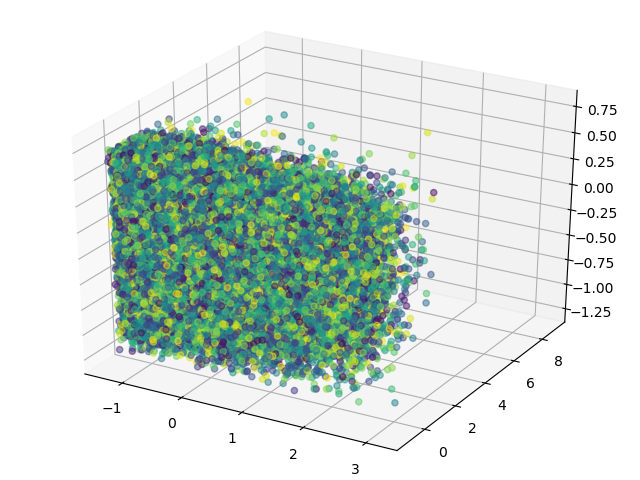
\includegraphics[scale=0.4]{./img/scatter}
  \caption{Input data: $5 \times 10^{4}$ entries.}
\end{center}
\end{figure}
\begin{itemize}
\item covariance matrix of size $5.10^{4} \times 5.10^{4}$, symmetric and double precision: full size in memory is $10 \mathrm{Go}$.
\end{itemize}
}
\only<2|handout:3>{
\begin{figure}[H]
\begin{center}
  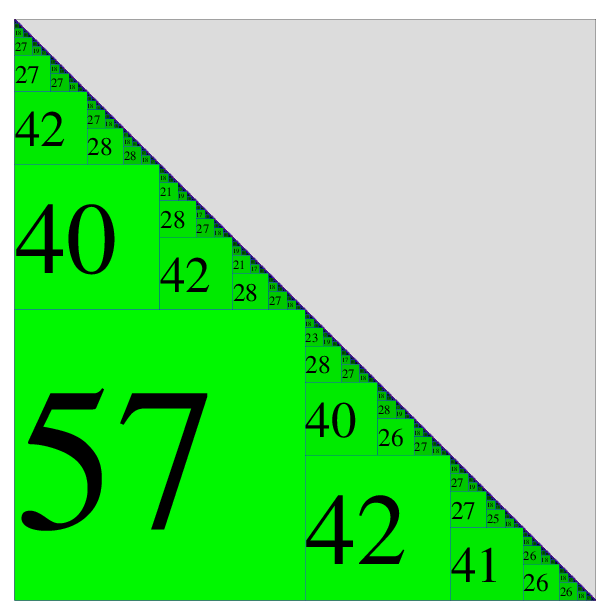
\includegraphics[scale=0.23]{./img/hmatrix_assembled}
  \caption{Lower part of the covariance matrix: rank map.}
\end{center}
\end{figure}

\begin{itemize}
\item memory: $167\mathrm{Mo}$ (compression ratio: 1.67\%);
\item assembly time: $11.83\mathrm{s}$
\end{itemize}

}
\only<3|handout:3>{
\begin{figure}[H]
\begin{center}
  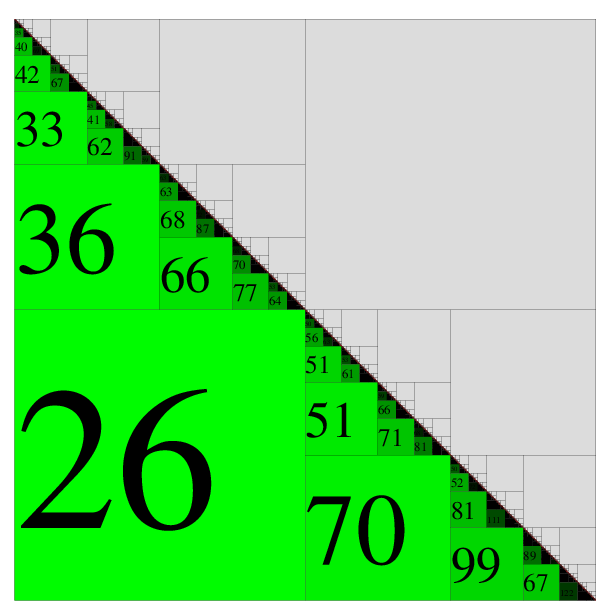
\includegraphics[scale=0.23]{./img/hmatrix_factorized}
  \caption{Cholesky factor: rank map.}
\end{center}
\end{figure}
\begin{itemize}
\item memory: $263\mathrm{Mo}$ (compression ratio: 2.63\%);
\item Cholesky time: $17.84\mathrm{s}$
\end{itemize}
}

\end{frame}

\begin{frame}
\frametitle{Gaussian process}
\begin{figure}[H]
\begin{center}
  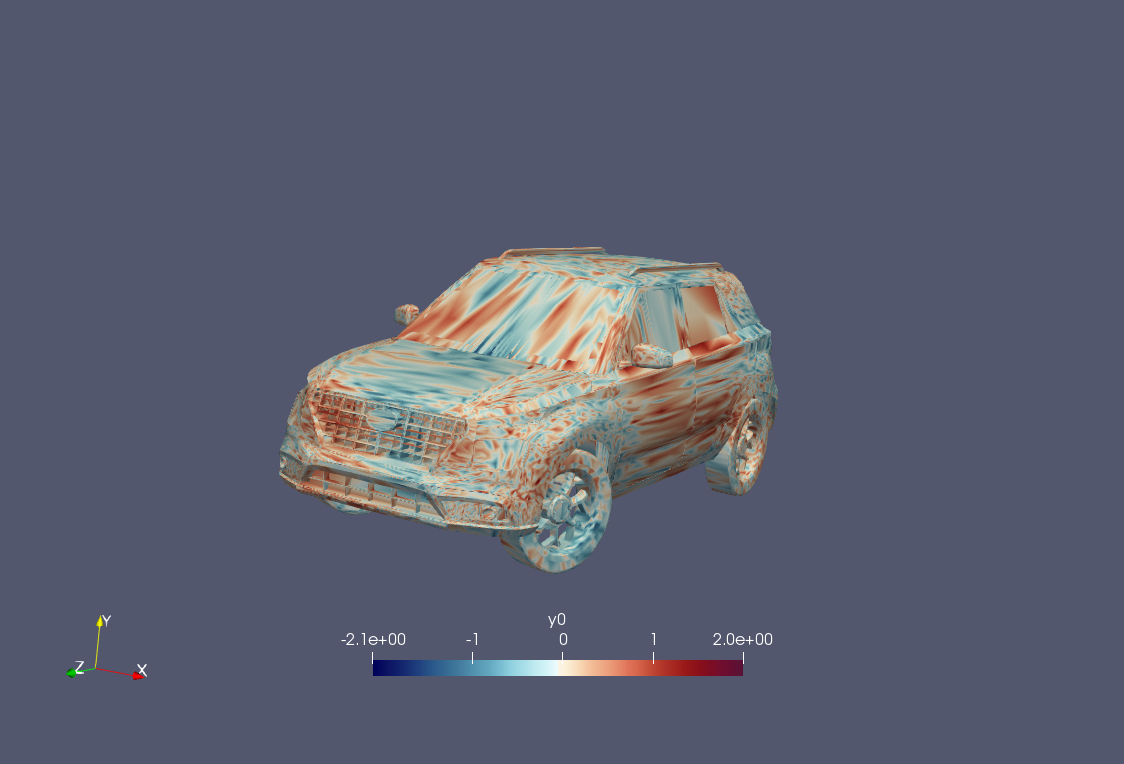
\includegraphics[scale=0.15]{./img/voiture}
  \caption{A Gaussian process on a Hyundai FEM mesh}
\end{center}
\end{figure}
\begin{itemize}
\item $144966$ vertices;
\item squared exponential covariance kernel.
\item Build, Cholesky factorization and trajectory generation in 118s.
\end{itemize}
\end{frame}


%% part 4: conclusion
\section{Conclusions \& perspectives}
\begin{frame}
\frametitle{Summing up the $\mathcal{H}$-matrices method}
\begin{itemize}
\item Three key components for assembling a $\mathcal{H}$-matrix: 
\begin{itemize}
  \item The clustering of degrees of freedom (e.g. geometric);
  \item An admissibility condition = which block to compress;
  \item A fast on-the-fly algorithm to assembly low-rank admissible blocks.
\end{itemize}
\item An algebra on $\mathcal{H}$-matrices: 
\begin{itemize}
\item Multiplications and additions of $\mathcal{H}$-matrices;
\item Fast factorization of an $\mathcal{H}$-matrix with the same structure :
\begin{itemize}
\item Fast direct solver;
\item Good preconditioner for iterative solver.
\end{itemize}
\end{itemize}
\end{itemize}
\end{frame}


\begin{frame}
\frametitle{Conclusion}
\begin{itemize}
  \item The \hmat framework is an enabler for many statistics problems;
  \item Sequential solver is freely available through OpenTurns;
  \item Efficient parallel solver through licensing (contact Airbus \& Imacs).
\end{itemize}
\end{frame}



\end{document}

